\chapter{University admission practices}\label{chap:4}

University admissions are lightly regulated, and in practice primarily focus on academic ability, rather than other factors that also affect completion prospects.

Universities are required by law to only admit students with the academic preparation needed for the course. All universities have policies on the minimum academic achievement required for admission. Most universities say that prospects for success are a selection principle. But a substantial minority of admitted students, one-in-five, have characteristics that put them at high risk of not completing their course. Most of them enrol part-time. Universities rarely scrutinise whether part-time students can put in the work necessary to complete their course.

\section{Legal requirements on admissions}\label{sec:4.1}

Universities have substantial autonomy over their admission requirements, although within legal minimum standards. In 2012 the government introduced `threshold standards' that all higher education providers must meet. These include admission standards. The Tertiary Education Quality and Standards Agency (TEQSA) is responsible for ensuring that the standards are met.

The first version of the threshold standards applied between 2012 and 2016. These required universities and other higher education providers to check that prospective students had `adequate prior knowledge and skills to undertake the course of study successfully'.\footcite[][15]{DIICCSRTE2013c} The latest standards, which took effect on 1 January 2017, contain a similar provision. Providers need to `ensure that admitted students have the academic preparation and proficiency in English needed to participate in their intended study'.

The new threshold standards also contain a potentially important addition: `\ldots{} and no known limitations that would be expected to impede {[}the student's{]} progression and completion'.\footcite[][3]{DepartmentofEducationandTraining2015n} 
This requires a more holistic view of possible impediments to success in higher education than just academic preparation. It can include orientation-type issues covered in the standards; for example that students know about and have access to support services they may need.

The evidence in this report shows that studying part-time, and especially studying a low number of subjects, should also be regarded as a known limitation that impedes progression and completion. Continuous part-time study, especially combined with other risk factors, makes completion unlikely. However, this is not the way either TEQSA or the universities interpret the standards (the role of TEQSA is discussed further in \Chapref{chap:7}).

\section{Admissions in practice}\label{sec:4.2}

Almost every university policy on admission has the applicant's prospect of success as a selection principle.\footnote{Based on desktop research in January 2018.} An acceptable level of risk is not stated, but the main tools for managing it are various measures of academic preparation.

                % Figure 20
                \begin{figure}
                    \caption{The higher-risk student group share of commencing enrolments has increased\label{fig:20}}%
                    \units{Commencing bachelor-degree students, per cent}
                    \includegraphics[page=26]{atlas/selection_chartdeck.pdf} 
                    \noteswithsource{`Low ATAR' is defined as students with an ATAR below 60, measured against the total number of domestic bachelor enrolments with an ATAR\@.}
                    {Grattan analysis of \textcite{DepartmentofEducationandTraininga}}
                \end{figure}

For school leavers, most universities use secondary education, and usually ATAR, as the main admission criteria.\footnote{The statistics on this subject have some issues: \textcite{Cherastidtham2018}. 
However between 2010 and 2016, 90 per cent of school-leaver entrants have an ATAR recorded in the enrolment data. Three-quarters of school-leaver entrants had a valid ATAR recorded and used secondary education as their basis of admission: \textcite{DepartmentofEducationandTraininga}.} Some courses also require prerequisite subjects in addition to English, which is necessary for an ATAR and which also is used to meet the standard on language proficiency.

For the most part, the standards and prospects for success are irrelevant to the ATARs required for admission. Instead, ATAR levels are typically set by the admissions market, with high-demand courses typically requiring ATARs that are well above the levels that would raise any concerns about risk of non-completion (\Cref{subsec:3.1.1}). ATAR is used as a fair and efficient way of allocating scarce student places, not to protect prospective students from a poor choice.\footnote{Universities require lower ATARs, or allocate bonus ATAR ranks for selection purposes, for students from disadvantaged backgrounds. A number of studies have shown that ATAR under-predicts their academic performance compared to other students with the same ATAR, for example: \textcites[][]{Li2014}[][]{Messinis2015a}.} Half of school leavers commencing university have ATARs above 80.

Although most ATAR course admission requirements are not related to any inherent minimum academic ability needed to do the course, many universities nominate a minimum ATAR, either overall or for particular courses. The minimum ATAR at several universities is between 50 and 60, indicating a willingness to take relatively high-risk students.

The proportion of commencing domestic bachelor-degree students being admitted with lower ATARs has trended up, as \Cref{fig:20} shows. The share of below-60 ATAR students grew from about 5 per cent in 2008 to more than 8 per cent in 2016.

For applicants seeking entry based on their previous higher education experience -- a growing share of new entrants -- universities typically use past academic performance, such as a grade point average (GPA). ATAR can often also be used if it is recent. Some universities let applicants use whichever of their GPA and ATAR is better.

The data used in the analysis for \Chapref{chap:3} does not include GPA, but failed subjects would lower a student's GPA. \Cref{subsec:3.1.1} showed that students with previous failed subjects are less likely to complete. About 5 per cent of commencing students failed at least one subject the previous year.\footcite{DepartmentofEducationandTraining2017n} 
Some universities have specific policies for these students. For example, the University of Tasmania requires applicants who have failed some subjects to undergo an extra review before an offer can be made.\footcite{UniversityofTasmania2018}

Students who repeatedly fail half or more of their subjects are likely to face exclusion from their university for unsatisfactory progress. Universities often impose a delay of 12 months before accepting another application from an excluded student. Once the waiting period ends, some universities require students to demonstrate how and why their chance of success in the course has improved.\footnote{For example  \textcites[][9]{UTS2016}[][8]{UniversityofMelbourne2017}[][]{Monash}.} 
Of all the admission criteria, this is the one that most carefully examines whether prospective students have a reasonable prospect of completing their degree.


Although ATAR gets most attention in public discussion about university admissions, part-time study is a more significant issue. The non-completion risk of studying few subjects a year is higher than having a low ATAR, and the proportion of students affected is larger. Part-time students grew from 15 per cent of commencing enrolments in 2011 to 18 per cent in 2015, before declining slightly in 2016 (\Cref{fig:20}). But part-time enrolment seems to get little attention during the admissions process.

A small number of courses offer full-time enrolment only, but generally students can freely choose to study part-time. A few universities recommend guidance from a program administrator. The main restriction on part-time study is the maximum time allowed to complete a degree. Typically, students have seven to ten years to complete a bachelor degree, depending on course and university. Some universities have formulas, such as twice the standard degree length for a full-time student, plus one or two years. Only some universities clearly signal maximum times in materials aimed at prospective students.

\section{High-risk students}\label{sec:4.3}

Mainly due to part-time study, a substantial minority of commencing students are at high risk of not completing a degree. Based on the risk analysis described in \Chapref{chap:3}, of the students commencing bachelor degrees in public universities in 2015, one in five -- more than 50,000 students -- are more likely to drop out than to complete their course within eight years. And nearly one in ten -- about 25,000 students -- have a non-completion risk of more than 70 per cent (\Cref{fig:21}).

Most high-risk students study part-time, as \Cref{fig:22} shows. Among students who are more likely to drop out than to complete, more than 80 per cent take four subjects or fewer in their first year. Less than 5 per cent of students who study more than six subjects are high risk.

Low ATAR is another major risk factor. As discussed in \Cref{subsec:3.1.1}, students with an ATAR below 60 face about double the non-completion risk as those with an ATAR of 90 or more.

Increased numbers of part-time and low-ATAR students help explain why overall non-completion rates are increasing (\Vref{sec:1.3}).

                % Figure 21
                \begin{figure}
                    \caption{One in five students is more likely to drop out of university than complete their course\label{fig:21}}%
                    \units{Commencing bachelor-degree domestic students, 2015, per cent}
                    \includegraphics[page=27]{atlas/selection_chartdeck.pdf} 
                    \notewithsource{For details on the modelling techniques, see the background paper, \textcite{Cherastidtham2018a}.}
                    {Grattan analysis of \textcite{DepartmentofEducationandTraininga}}
                \end{figure}


                % Figure 22
                \begin{figure}
                    \caption{Of students who are more likely to drop out than complete, more than 80 per cent study part-time\label{fig:22}}%
                    \units{Commencing bachelor-degree domestic students, 2015, per cent}
                    \includegraphics[page=28]{atlas/selection_chartdeck.pdf} 
                    \noteswithsource{Rounding means the percentages do not add up to 100. See \Cref{fig:21}.}
                    {See \Cref{fig:21}}
                \end{figure}


